\documentclass[10pt,a4paper]{article}
\usepackage[utf8]{inputenc}
\usepackage[T1]{fontenc}
\usepackage[ngerman]{babel}
\usepackage{amsmath}
\usepackage{amsfonts}
\usepackage{amssymb}
\usepackage{graphicx}


\author{Gruppe 02}
\title{Pflichtenheft}
\begin{document}
% Title Page foo
\maketitle
\newpage

% Inhaltsverzeichniss
\tableofcontents
\newpage

% Sections
\section{Einführung}
\subsection{Überblick}
\subsection{Technologien}
\section{System \"Ubersicht}

\subsection{Komponentendiagramm}

\begin{figure}[H]
  \centering
  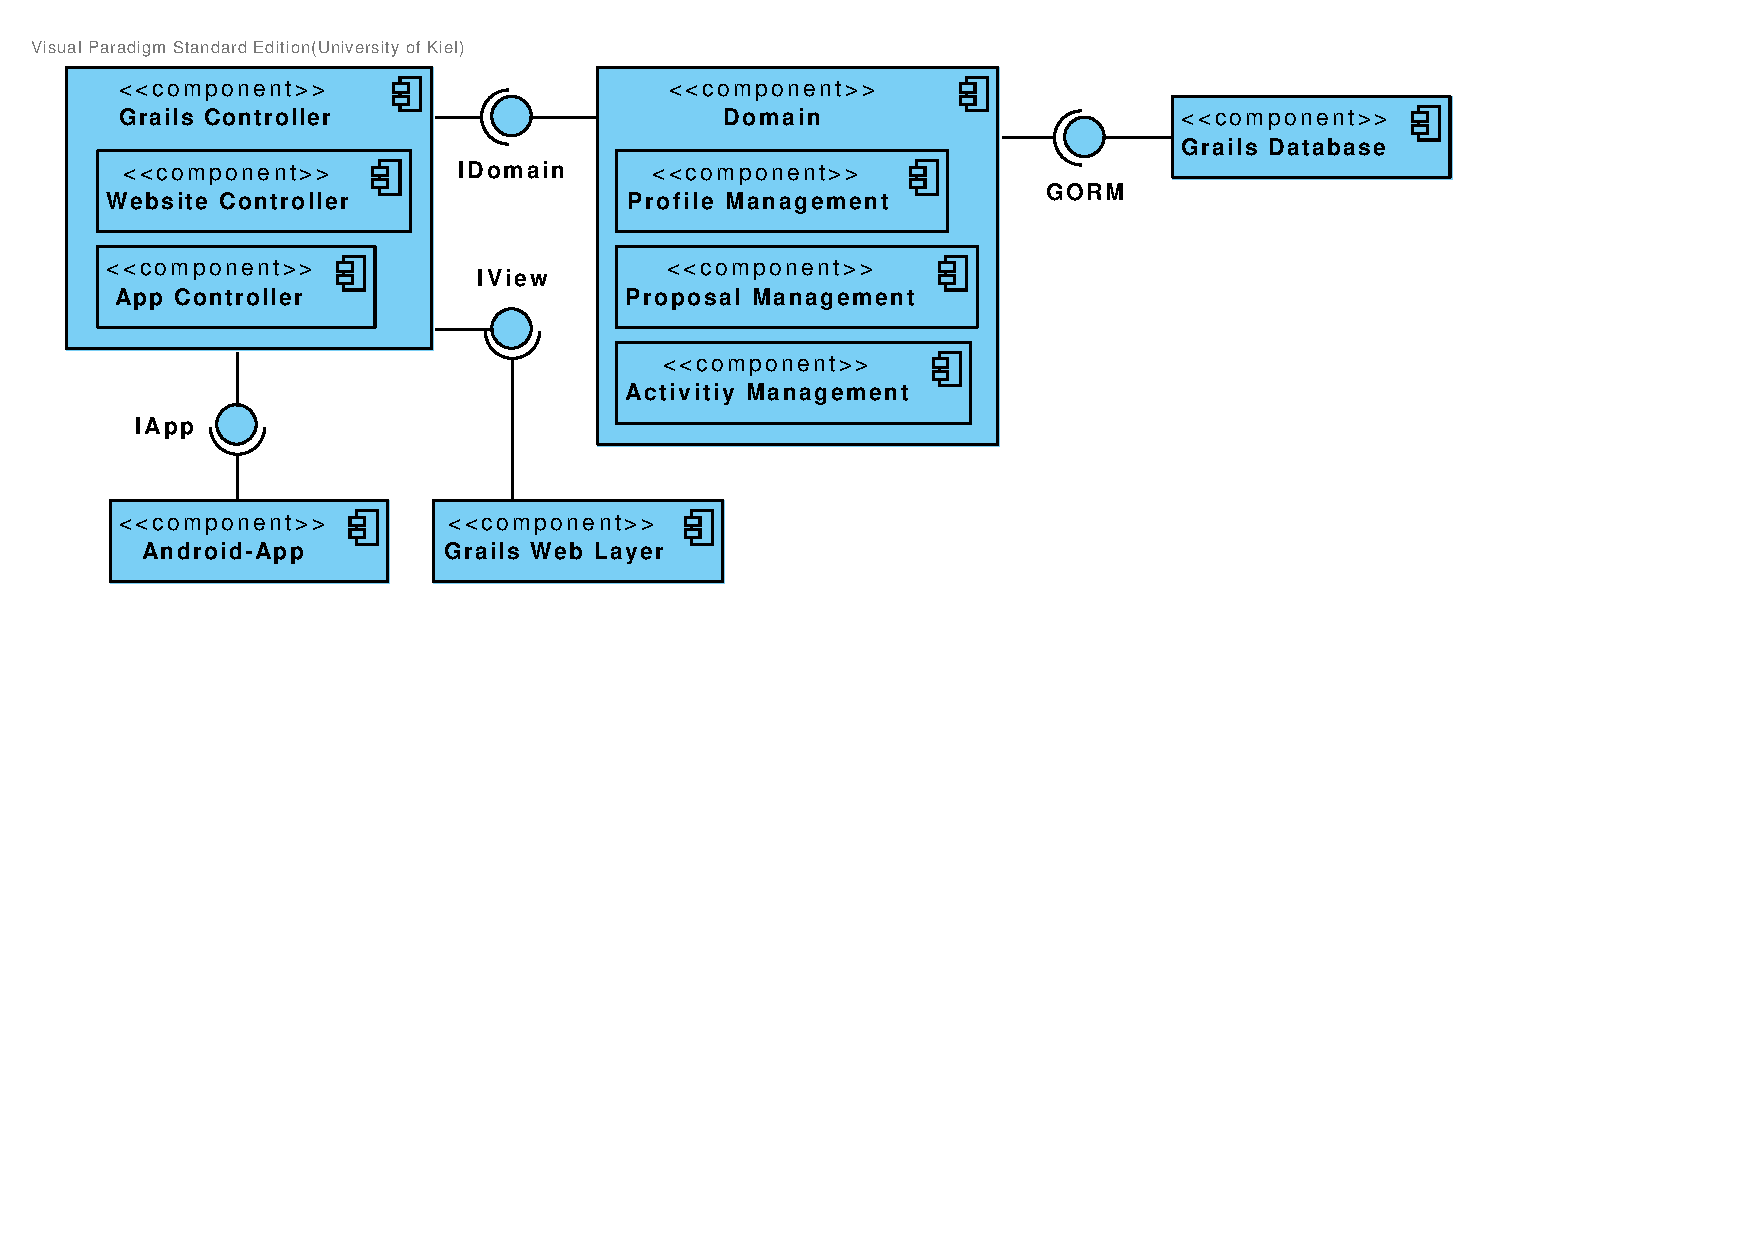
\includegraphics[width=\textwidth, clip]{gfx/component_diagram}
  \caption{Komponentendiagramm}
\end{figure}

\paragraph{Grails Database} Die Grails Database Komponente ist die
zentrale Datenbank, die auf dem Server liegt und s\"amtliche Daten
enth\"alt, auf die \"uber das durch \emph{Grail's Object
  Relational Mapping} (GORM) bereitgestellte Interface zugegriffen werden kann.

\paragraph{Domains} Die Domain Komponente ist die Modell
Repr\"asentation der Daten in der Datenbank. Der Zugriff erfolgt
\"uber das IDomain Interface. Die Domain Komponenten ist unterteilt in
die Subkomponenten \emph{Profile Management}, \emph{Proposal
  Management} und \emph{Activity Management}. Das Profile Management
ist zuständig für die Verwaltung der Modellrepräsentation von Team-
und Benutzerprofilen. Das Proposal Managment ist zuständig für die
Verwaltung der Modellrepräsentation von (Aktivitäts-) Vorschlägen. Die
Komponente Activity Management ist zuständig für die Verwaltung der Modellrepräsentation von Aktivitäten.

\paragraph{Grails Web Layer} Die Grails Web Layer Komponente kommuniziert mit dem Grails Controller \"uber das IView Interface und stellt die GSP Dateien zur Verf\"ugung, die das Layout der Webseite spezifizieren.

\paragraph{Grails Controller} Die Controller Komponente besteht aus den einzelnen Controllern f\"ur Webseite und Android App und ist zust\"andig f\"ur die Verarbeitung s\"amtlicher Daten und Anfragen, die \"uber die IApp, IDomain und IView Schnittstellen kommuniziert werden.

\paragraph{Android App} Die Android App, dient in erster Linie zur Repr\"asentation der Daten vom Server auf Mobilger\"aten. Sie kommuniziert \"uber das IApp Interface mit dem Controller.

\subsection{Verteilungsdiagramm}

\subsubsection{Android-Gerät}
Das Android-Gerät ist das Arbeitswerkzeug für die Benutzer. Auf dem Gerät ist eine native Android-Applikation installiert, mit der Daten eingegeben und abgerufen werden können. Der Benutzer muss bereits registriert sein, um die Applikation nutzen zu können.
\subsubsection{Computer}
Benutzer können mit Hilfe eines Computers über einen Webbrowser auf eine Webseite zugreifen, welche, nach erfolgreichem einloggen, verschiedene Funktionen zur Aktivitäts- und Profilverwaltung anbietet.Des Weiteren können hier auch anonymisierte Statistiken angezeigt und diese statistischen Daten exportiert werden.
\subsubsection{Server}
Der Server stellt die eben erwähnte Webseite bereit. Hier werden gegebenenfalls Datenanfragen von den Android-Geräten verarbeitet.
\subsection{Paketdiagramm}
\section{Ordner Struktur}
% TODO Beschreibung der Ordnerstruktur
\section{Klassen}
	\paragraph{Informationen}
	Generell sind die Klassen aufgeteilt in unterschiedliche Bereiche. Zun\"achst die grobe Unterteilung in Klassen, die in Bezug zur Website stehen und Klassen mit Bezug zur Android App, dann die Klassen der Website weiter verfeinert in
	\begin{itemize}
		\item Modellklassen: Klassen, die sich auf die Persistenz beziehen, wie beispielsweise die verschiedenen Objekte, die in der Datenbank gespeichert werden.
		\item Controllerklassen: Klassen, die dazu dienen Nutzeranfragen und Darstellungen zu verwalten, jedoch auf die Datenbank nur lesend zugreifen. Diese Klassen sind zudem daf\"ur verantwortlich die Anzeige (mittels index() Methode) der jeweiligen Daten, auf die sie sich beziehen, zu steuern. (Dieser Umstand trifft auf alle Controllerklassen zu und wird daher in der Beschreibung der einzelnen Klassen sowie bei den Methoden nicht jedes Mal explizit erw\"ahnt.)
		\item Serviceklassen: Klassen, die Methoden enthalten, die die Datenpersistenz beeinflussen, also mit speicherndem und \"anderndem Zugriff. 
	\end{itemize}
	
\subsection{Website}

\subsubsection{Modellklassen}
	\paragraph{Activity}Enth\"alt alle Informationen \"uber eine Energiesparaktivit\"at, die von Benutzern erledigt werden kann.
		\begin{itemize}
			\item Attribute:
				\begin{itemize}
					\item description: Ein String, der die Aktivit\"at beschreibt.
					\item points: Eine nat\"urliche Zahl von 1 bis 5, die angibt wie viele Punkte die Erledigung der Aktivit\"at wert ist.
					\item duration: Eine Zeitangabe, die angibt, wie lange die Aktivit\"at nach Ausf\"uhrung gesperrt ist, bevor sie wieder erledigt werden kann.
				\end{itemize}
		\end{itemize}
	\paragraph{CompletedActivity}Beinhaltet Informationen \"uber von Benutzern abgeschlossene Aktivit\"aten.
		\begin{itemize}
			\item Attribute:
			\begin{itemize}
				\item date: Ein DateTime Objekt, das angibt, wann die Aktivit\"at erledigt wurde.
			\end{itemize}
		\end{itemize}
	\paragraph{Profile}Verwaltet Informationen bez\"uglich der Team- und Benutzerprofile.
		\begin{itemize}
			\item Attribute:
			\begin{itemize}
				\item avatar: Das Profilbild, gespeichert als Byte Array.
				\item name: Der Name des Benutzers oder Teams des jeweiligen Profils.
				\item avatarType: Das Datenformat des Profilbildes, als String gespeichert.
				\item blocked: Ein boolescher Wert, der angibt, ob das Profil gegenw\"artig gesperrt ist.
			\end{itemize}
		\end{itemize}
	\paragraph{User}Erweitert die Klasse Profile um die pers\"onlichen Informationen eines Benutzers und dient Apache Shiro zur Authentifikation.
		\begin{itemize}
			\item Attribute:
			\begin{itemize}
				\item email: Die E-Mail Adresse eines Benutzers, gespeichert als String.
				\item passwordHash: Die als String gespeicherte Hash-Repr\"asentation des Passworts eines Benutzers.
				\item title: Der akademische Titel eines Benutzers als String.
				\item emailNotification: Ein boolescher Wert, der angibt, ob der Benutzer E-Mail Benachrichtigungen erh\"alten m\"ochte oder nicht.
			\end{itemize}
		\end{itemize}
	\paragraph{Team}Erweitert die Klasse Profile und beinhaltet die Informationen eines Teams.
	\paragraph{Role}Enth\"alt Informationen \"uber die verschiedenen Rollen auf der Website, die den Zugriff auf bestimmte Inhalte einschr\"anken.
	\paragraph{Comment}Enth\"alt Informationen zu Kommentaren bez\"uglich Energiesparvorschl\"agen.
		\begin{itemize}
			\item Attribute:
			\begin{itemize}
				\item text: Ein String, der den Text des Kommentars enth\"alt.
				\item rating: Eine nat\"urliche Zahl zwischen 1 und 5, die eine Bewertung des kommentierten Vorschlags darstellt.
			\end{itemize}
		\end{itemize}
	\paragraph{Proposal}Beinhaltet Informationen zu einem durch einen Benutzer eingereichten Energiesparvorschlag.
		\begin{itemize}
			\item Attribute:
			\begin{itemize}
				\item description: Ein String, der den Energiesparvorschlag beschreibt.
				\item points: Eine nat\"urliche Zahl von 1 bis 5, die angibt wie viele Punkte die Erledigung der vorgeschlagenen Aktivit\"at wert sein soll.
			\end{itemize}
		\end{itemize}
	\paragraph{Institute}Die Klasse, die Informationen \"uber die Institutszugeh\"origkeit eines Benutzers beinhaltet.
		\begin{itemize}
			\item Attribute:
			\begin{itemize}
				\item name: Der Name des Instituts als String.
			\end{itemize}
		\end{itemize}
	\paragraph{Message}Die Klasse, die Informationen \"uber Nachrichten speichert, die an Benutzer gesendet werden können.
	\paragraph{TeamInvite}Erweitert Message und enth\"alt Informationen bez\"uglich einer Teameinladung f\"ur einen Benutzer.
	\paragraph{ActivityNotification}Erweitert die Klasse Message und enth\"alt Informationen \"uber eine allgemeine Erinnerungsnachricht an einen Benutzer.
	\paragraph{SpecificActivityNotification}Erweitert Message und enth\"alt Informationen \"uber eine Erinnerungsnachricht an einen Benutzer, eine spezielle Aktivit\"at betreffend.

\subsubsection{Controllerklassen}
	\paragraph{AuthController}Verwaltet das An- und Abmelden sowie das Registrieren von Benutzern auf der Website.
		\begin{itemize}
			\item Methoden:
			\begin{itemize}
				\item login(): Diese Funktion steuert die Anmeldung von Benutzern.
				\item logout(): Mit dieser Funktion k\"onnen sich Benutzer von der Anwendung wieder abmelden und so ihre aktuelle Sitzung beenden.
				\item register(): Diese Funktion dient dazu, Benutzer im System zu registrieren.
			\end{itemize}
		\end{itemize}
	\paragraph{UserController}Die Klasse, die die Einstellungen bez\"uglich eines Benutzerprofils verwaltet.
		\begin{itemize}
			\item Methoden:
			\begin{itemize}
				\item edit(): Diese Methode erm\"oglicht dem Benutzer die Bearbeitung seiner pers\"onlichen Einstellungen.
				\item uploadAvatar(): Die Methode, die ein Benutzer verwendet, um ein neues Profilbild hochzuladen.
				\item avatarImage(): Die Methode, die das Profilbild in ein Bildformat konvertiert.
				\item show(): Die Methode, die das Profil eines Benutzers anzeigt.
				\item joinTeam(): Methode, die aufgerufen wird, wenn ein Benutzer eine Teameinladung annimmt oder einem bestehenden Team beitritt.
				\item newTeam(): Eine Methode, die es einem Benutzer erm\"oglicht ein neues Team zu erstellen.
				\item changePassword(): Die Methode, die aufgerufen wird, wenn ein Benutzer sein Passwort \"andern m\"ochte.
				\item changeEmailNotification(): Die Methode, die die E-Mail Benachrichtigungseinstellungen eines Benutzers \"andert.
			\end{itemize}
		\end{itemize}
	\paragraph{TeamController}Verwaltet die Einstellungen bez\"uglich eines Teamprofils.
		\begin{itemize}
			\item Methoden:
			\begin{itemize}
				\item edit(): Diese Methode erm\"oglicht dem Benutzer die Bearbeitung der Einstellungen seines Teams.
				\item uploadAvatar(): Die Funktion, die ein Benutzer aufruft, um ein neues Profilbild f\"ur sein Team hochzuladen.
			\end{itemize}
		\end{itemize}
	\paragraph{AdminController}Die Klasse, die s\"amtliche adminspezifische Anfragen erm\"oglicht und verwaltet.
		\begin{itemize}
			\item Methoden:
			\begin{itemize}
				\item listUsers(): Methode, die eine Liste aller Benutzer aus der Datenbank holt und diese anzeigt.
				\item listTeams(): Methode, die eine Liste aller Teams aus der Datenbank holt und diese anzeigt.
				\item listProposals(): Methode, die eine Liste aller Energiesparvorschl\"age aus der Datenbank holt und diese anzeigt.
				\item listActivities(): Methode, die eine Liste aller Aktivit\"aten aus der Datenbank holt und diese anzeigt.
				\item editActivity(): Die Funktion, die dem Admin erm\"oglicht, eine Aktivit\"at zu bearbeiten.
				\item editProposal(): Die Funktion, die dem Admin erm\"oglicht, einen Energiesparvorschlag zu bearbeiten.
				\item editTeam(): Die Funktion, die dem Admin erm\"oglicht, ein Team zu bearbeiten.
				\item editUser(): Die Funktion, die dem Admin erm\"oglicht, einen Benutzer zu bearbeiten.
				\item blockUser(): Die Methode, mit der ein Benutzer gesperrt wird.
				\item blockTeam(): Die Methode, mit der ein Team (und damit automatisch alle Benutzer, die Mitglieder des Teams sind) gesperrt werden.
				\item unblockUser(): Die Methode, mit der ein Benutzer reaktiviert wird.
				\item unblockTeam(): Die Methode, mit der ein Team (und damit alle Mitglieder) reaktiviert werden.
				\item deleteUser(): Methode, mit der der Admin einen Benutzer l\"oscht.
				\item deleteTeam(): Methode, mit der der Admin ein Team l\"oscht.
			\end{itemize}
		\end{itemize}
	\paragraph{AppController}Die Klasse, die f\"ur die Kommunikation zwischen Server und App verantwortlich ist und Anfragen der App verarbeitet.
		\begin{itemize}
			\item Methoden:
			\begin{itemize}
				\item getRankingTeams(): Methode, die die aktuelle Team-Rangliste (inklusive einzelner Benutzer ohne Team) aus der Datenbank liest und als JSON Objekt an die App sendet.
			\end{itemize}
		\end{itemize}
	\paragraph{LandingController}Steuert die Benutzung der Landing Page (Hauptseite).
	\paragraph{RankingController}Die Klasse, die die Benutzung der Ranglistenseite steuert.
	\paragraph{ActivityController}Verwaltet die Benutzung der Aktivit\"atenseite und erm\"oglicht beispielsweise das erledigen von Aktivit\"aten.
		\begin{itemize}
			\item Methoden:
			\begin{itemize}
				\item completeActivity(): Die Methode, die eine Aktivit\"at f\"ur einen Benutzer als erledigt markiert und daf\"ur sorgt, dass ihm die entsprechenden Punkte gutgeschrieben werden.
			\end{itemize}
		\end{itemize}
	\paragraph{ProposalController}Die Klasse, die alle Aktionen rund um Energiesparvorschl\"age und die entsprechende Website verwaltet.
		\begin{itemize}
			\item Methoden:
			\begin{itemize}
				\item new(): Die Methode, die einen neuen Energiesparvorschlag anlegt.
				\item comment(): Mit dieser Funktion kann ein Benutzer einen neuen Kommentar zu einem Energiesparvorschlag abgeben.
				\item list(): Zeigt eine \"Ubersicht \"uber alle Energiesparvorschl\"age.
				\item view(): Zeigt die Energiesparvorschl\"age an.
			\end{itemize}
		\end{itemize}
	\paragraph{ProfileController}Verwaltet die Profilseite eines Benutzers oder Teams.
		\begin{itemize}
			\item Methoden:
			\begin{itemize}
				\item viewPage(): Speichert den Webseitenaufruf eines Benutzers.
			\end{itemize}
		\end{itemize}
	\paragraph{StatisticsController}Verwaltet die Auswahl und Erstellung von Statistiken.
		\begin{itemize}
			\item Methoden:
			\begin{itemize}
				\item exportToCsv(): Startet einen Download der Statistiken als .csv Datei.
			\end{itemize}
		\end{itemize}

\subsubsection{Serviceklassen}
	\paragraph{ProposalService}Die Klasse, die neue Energiesparvorschl\"age und Kommentare dazu erm\"oglicht.
		\begin{itemize}
			\item Methoden:
			\begin{itemize}
				\item addComment(commentText : String, rating : int, author : Subject, proposalId : long): Methode, die dem durch die proposalId gegebenen Energiesparvorschlag einen Kommentar hinzuf\"ugt.
				\item addProposal(description : String, points : int, author : Subject): Speichert einen neuen Energiesparvorschlag in der Datenbank.
			\end{itemize}
		\end{itemize}
	\paragraph{ActivityService}Erm\"oglicht verschiedene Aktionen zu Aktivit\"aten auszuf\"uhren.
		\begin{itemize}
			\item Methoden:
			\begin{itemize}
				\item completeActivity(activityId : long, subject : Subject): Methode, die die durch die activityId gegebene Aktivit\"at als erledigt markiert und die entsprechenden Punkte auf die Punktzahl des durch das Subjekt gegebenen Benutzers in der Datenbank addiert.
				\item addToFavorites(activityId : long, subject : Subject): Die Funktion, die eine Aktivit\"at in den Favoriten eines Benutzers speichert.
				\item removeFromFavorites(activityId : long, subject : Subject): Die Methode, die eine Aktivit\"at aus den gespeicherten Favoriten eines Benutzers l\"oscht.
			\end{itemize}
		\end{itemize}
	\paragraph{MessageService}Die Klasse, die das Versenden von Teameinladungen und Erinnerungsnachrichten ausf\"uhrt.
		\begin{itemize}
			\item Methoden:
			\begin{itemize}
				\item inviteUserToTeam(receiverId : long, subject : Subject): Die Methode, die einem anderen Benutzer eine Teameinladung sendet.
				\item remindUser(receiverId : long): Die Methode, die einem Benutzer eine generelle Erinnerungsnachricht sendet.
				\item remindUser(receiverId : long, activityId : long): Methode, die einem Benutzer eine Erinnerungsnachricht bez\"uglich einer bestimmten Aktivit\"at sendet.
			\end{itemize}
		\end{itemize}
	\paragraph{SettingsService}Die Klasse, die alle Daten- und Einstellungs\"anderungen eines Benutzers ausf\"uhrt.
		\begin{itemize}
			\item Methoden:
			\begin{itemize}
				\item setName(title : String, firstName : String, lastName : String, subject : Subject): Speichert den Namen eines Benutzers in der Datenbank.
				\item setPassword(password1 : String, password2 : String, subject : Subject): Speichert das Passwort eines Benutzers als Hash in der Datenbank.
				\item setAvatar(avatar : def, subject : Subject): Speichert das Profilbild eines Benutzers als Byte Array in der Datenbank.
				\item setInstitute(instituteID : long, subject : Subject): Speichert das Institut eines Benutzers in der Datenbank.
				\item setTeam(teamId : long, subject : Subject): Speichert das Team eines Benutzers in der Datenbank.
				\item setEmailNotification(emailNotification : boolean, subject : Subject): Speichert die Einstellungen bez\"uglich E-Mail Benachrichtigung eines Benutzers in der Datenbank.
				\item createTeamAndJoin(name : String, avatar : def, subject : Subject): Speichert ein neues Team in der Datenbank und das Team zudem als Team des Erstellers.
			\end{itemize}
		\end{itemize}
	\paragraph{TeamService}Erm\"oglicht die \"Anderung des Avatars und Namens eines Teams.
		\begin{itemize}
			\item Methoden:
			\begin{itemize}
				\item setName(naem : String, teamId : long): Speichert den Namen eines Teams in der Datenbank.
				\item setAvatar(avatar : def, subject : Subject): Speichert das Profilbild eines Teams als Byte Array in der Datenbank.
			\end{itemize}
		\end{itemize}
	\paragraph{AdminService}F\"uhrt alle Administrator-spezifischen Operationen aus, die die Datenpersistenz ver\"andern.
		\begin{itemize}
			\item Methoden:
			\begin{itemize}
				\item createActivity(description : String, points : int, duration : Duration): Speichert eine neue Aktivit\"at in der Datenbank.
				\item createActivityFromProposal(description : String, points : int, duration : Duration, proposalId : long): Speichert eine neue Aktivit\"at in der Datenbank, l\"oscht anschließend den Energiesparvorschlag, dem diese entstammt und schreibt dem Autor des Vorschlags 2 Punkte gut.
				\item deleteActivity(activityId : long): L\"oscht eine Aktivit\"at aus der Datenbank.
				\item editActivity(activityId : long, description : String, points : int, duration : Duration): Ver\"andert eine bestehende Aktivit\"at in der Datenbank.
				\item deleteProposal(proposalId : long): L\"oscht einen Energiesparvorschlag aus der Datenbank.
				\item blockUser(userId : long): Setzt den blocked Wert eines Benutzers auf wahr.
				\item unblockUser(userId : long): Setzt den blocked Wert eines Benutzers auf falsch.
				\item deleteUser(userId : long): L\"oscht einen Benutzer aus der Datenbank.
				\item blockTeam(teamId : long): Setzt den blocked Wert eines Teams auf wahr.
				\item unblockTeam(teamId : long): Setzt den blocked Wert eines Teams auf falsch.
				\item deleteTeam(teamId : long): L\"oscht ein Team aus der Datenbank.
			\end{itemize}
		\end{itemize}
	\paragraph{PageViewService}Speichert die Seitenaufrufe der einzelnen URLs in der Datenbank.
		\begin{itemize}
			\item Methoden:
			\begin{itemize}
				\item viewPage(url : String): Speichert einen Seitenaufruf der gegebenen URL in der Datenbank.
			\end{itemize}
		\end{itemize}

\subsection{Android App}
Die Klassen in \emph{Activities}, \emph{Adapters} sowie die Klasse \emph{AccessServerTask} erweitern vordefinierte Android-Klassen. Hierdurch werden viele Methoden definiert, die die vordefinierten Methoden überschreiben, wie zum Beispiel \emph{onCreate} oder \emph{onDestroyView}. Diese werden im Klassendiagramm und der folgenden Beschreibung nicht explizit aufgeführt.
\subsubsection{Activities}
\paragraph{MainActivity} Die \emph{Activity}, die für die Darstellung der Hauptfunktionen zuständig ist. Das bedeutet in ihr wird die Navigation aufgerufen und die meisten Funktionen, die als \emph{Fragment} dargestellt werden.
\paragraph{LoginActivity} Die \emph{Activity}, über die die Anmeldung erfolgt.
\paragraph{SearchActivity} Dient zur Ausführung einer Suche und dem Anzeigen der Ergebnisse.
\paragraph{ProposalActivity} Dient zur Anzeige eines Energiesparvorschlags inklusive seiner Bewertungen und Kommentare. Ermöglicht außerdem das Bewerten und Kommentieren von Energiesparvorschl\"agen.
\paragraph{TeamProfilActivity} Zeigt das Profil eines Benutzers an.
\paragraph{UserProfilActivity} Zeigt das Profil eines Teams an.
\paragraph{MainFragment} Darstellung des Haupt-\emph{Fragments}.
\paragraph{MyProfilFragment} Zeigt das eigene Profil an.
\paragraph{RankinglistFragment} Zeigt das \emph{Fragment} für die Benutzer- bzw. Teamrangliste an.
\paragraph{TeamRankingsTabFragment} Zeigt die aktuelle Team-Rangliste an.
\paragraph{UserRankingsTabFragment} Zeigt die aktuelle Benutzer-Rangliste an.
\paragraph{ProposalFragment} Zeigt alle Energiesparvorschläge an.
\paragraph{NavigationFragment} Die Navigation innerhalb der Haupt-\emph{Activity}.

\subsubsection{Adapters}
\paragraph{FavoriteActivitiesAdapter} Zuständig für die Anzeige der favorisierten Aktivitäten. Von hier aus sollen auch Aktivitäten ausgeführt werden können, wenn sie angeklickt werden.
\paragraph{ActivitiesAdapter} Zuständig für die Anzeige aller Aktivitäten. Bei einem Klick auf eine Aktivität wird diese ausgeführt.
\paragraph{UserRankingsAdapter} Zuständig für die Anzeige der Benutzer-Rangliste. Bei einem Klick auf einen Benutzer soll eine \emph{UserProfilActivity} erstellt werden, in der der angeklickte Benutzer ausgeben wird.
\paragraph{TeamRankingsAdapter} Zuständig für die Anzeige der Team-Rangliste. Bei einem Klick auf ein Team soll eine \emph{TeamProfilActivity} erstellt werden, in der das angeklickte Team ausgeben wird.
\paragraph{ProposalsAdapter} Zuständig für die Anzeige der Energiesparvorschläge. Bei einem Klick auf einen Vorschlag soll eine \emph{ProposalActivity} erstellt werden, in der das angeklickte Team ausgeben wird.

\subsubsection{Tasks}
\paragraph{AccessServerTask} Eine Klasse, die eine abstrakter Serveranfrage darstellt. Alle Serveranfragen-Klassen erben von dieser Klasse und implementieren die abstrakten Methoden \emph{createServerRequest()} und \emph{handleServerResponse()} in welchen eine Server-Anfrage gestellt wird und eine Server-Antwort verarbeitet wird. Die Klasse kümmert sich um den Verbindungsaufbau, die Antwort und das Parsen der Daten, so dass die abgeleiteten Methoden sich nicht mehr darum kümmern müssen.
\paragraph{GetTeamProfileTask} Die Klasse, die dafür zuständig ist, ein Teamprofil vom Server zu laden und in der \emph{TeamProfilActivity} anzuzeigen.
\paragraph{GetUserProfileTask} Die Klasse, die dafür zuständig ist, ein Benutzerprofil vom Server zu laden und in der \emph{UserProfilActivity} bzw. im \emph{MyProfilFragment} anzuzeigen.
\paragraph{GetTeamRakingTask} Die Klasse, die dafür zuständig ist, das Team-Ranking vom Server zu holen und an den \emph{TeamRankingsAdapter} weiterzureichen.
\paragraph{GetUserRakingTask} Die Klasse, die dafür zuständig ist, das Benutzer-Ranking vom Server zu holen und an den \emph{TeamRankingsAdapter} weiterzureichen.
\paragraph{GetActivitiesTask} Die Klasse, die dafür zuständig ist, die Liste aller Aktivitäten vom Server zu holen und an den \emph{ActivitiesAdapter} weiterzureichen.
\paragraph{GetFavoriteActivitiesTask} Die Klasse, die dafür zuständig ist, die Liste der favorisierten Aktivitäten vom Server zu holen und im \emph{MainFragment} anzuzeigen.
\paragraph{GetProposalsTask} Die Klasse, die dafür zuständig ist, die Energiesparvorschläge vom Server zu holen und an den \emph{ProposalsAdapter} weiterzureichen.
\paragraph{GetProposalTask} Die Klasse, die dafür zuständig ist, einen konkreten Energiesparvorschlag vom Server zu laden und in der \emph{ProposalActivity} anzuzeigen.
\paragraph{SearchTask} Die Klasse, die dafür zuständig ist, eine Suchanfrage an den Server zu stellen und das Ergebnis in der \emph{SearchActivity} anzuzeigen.
\paragraph{DoActivityTask} Die Klasse, die dafür zuständig ist, dem Server mitzuteilen, dass ein Benutzer eine Aktivität ausgeführt hat.
\paragraph{CommentProposalTask} Die Klasse, die dafür zuständig ist, dem Server mitzuteilen, dass ein Benutzer einen Energiesparvorschlag bewertet oder kommentiert hat.

\subsubsection{Utils}
\paragraph{IoX} Klasse, die Methoden für generelles Input/Output bereitstellt. Das ist zum aktuellen Zeitpunkt nur die Methode \emph{readInputStream}, die einen \emph{InputStream} in einen String umwandelt.
\paragraph{ServerRequest} Klasse, die eine Serveranfrage modelliert. Eine Serveranfrage besteht aus einem Adressaten auf dem Server und aus der eigentlichen Anfrage. Die eigentliche Anfrage ist ein JSON-Objekt.

\section{Dynamisches Verhalten}

\subsection{Login/Registrierung}
%TODO Image here
\subsection{Aktivität erledigen}

\begin{figure}[H]
  \centering
  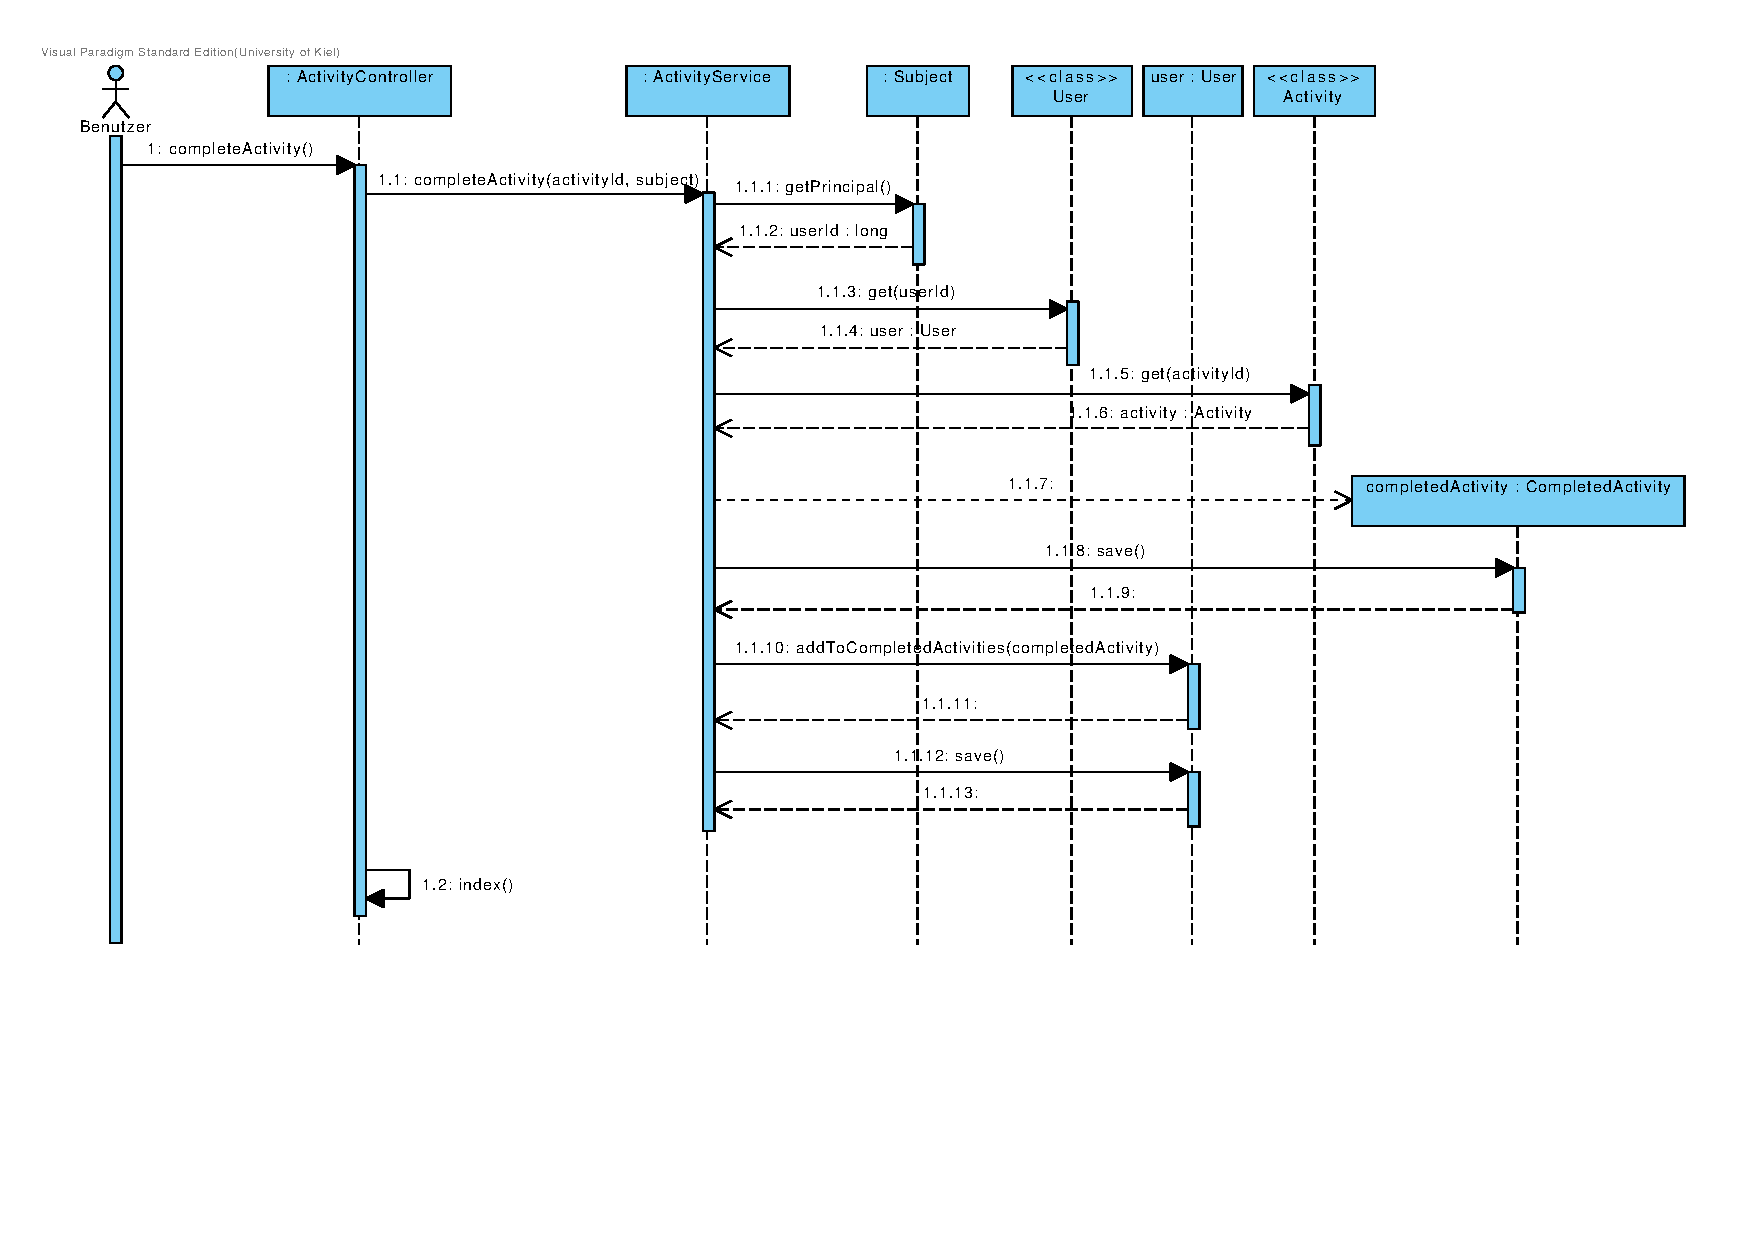
\includegraphics[width=\textwidth, clip]{gfx/aktivitaet_erledigen}
  \caption{Ein Team erstellen}
\end{figure}

Der eingeloggte Benutzer gelangt über einen Klick auf „Aktivitäten“
auf die Aktivitätenseite. Auf dieser findet er die Liste mit
Aktivitäten. Durch das Klicken auf die zu erledigende Aktivität werden
dem Benutzer die entsprechenden Punkte gutgeschrieben und die
erledigte Aktivität wird für den Benutzer gesperrt bis die festgelegte
Sperrphase abgelaufen ist. Der Benutzer wird dadurch außerdem wieder auf die
Aktivitätenseite zurück geleitet.

Alternativ ist das Erledigen favorisierter Aktivtäten auch auf der
Landingpage möglich.

\subsection{Rangliste ansehen}
%TODO Image here
Der eingeloggte Admin kann ein Team über einen speziellen Button, welcher die Funktion blockTeam(teamId) aufruft, sperren. Dabei wird das Team und nacheinander jedes einzelne Teammitglied gesperrt. Nachdem dies geschehen ist, tauchen auch das Team und deren Mitglieder nicht mehr in der Teilnehmerliste auf.\\

\subsection{Team erstellen}
\begin{figure}[H]
  \centering
  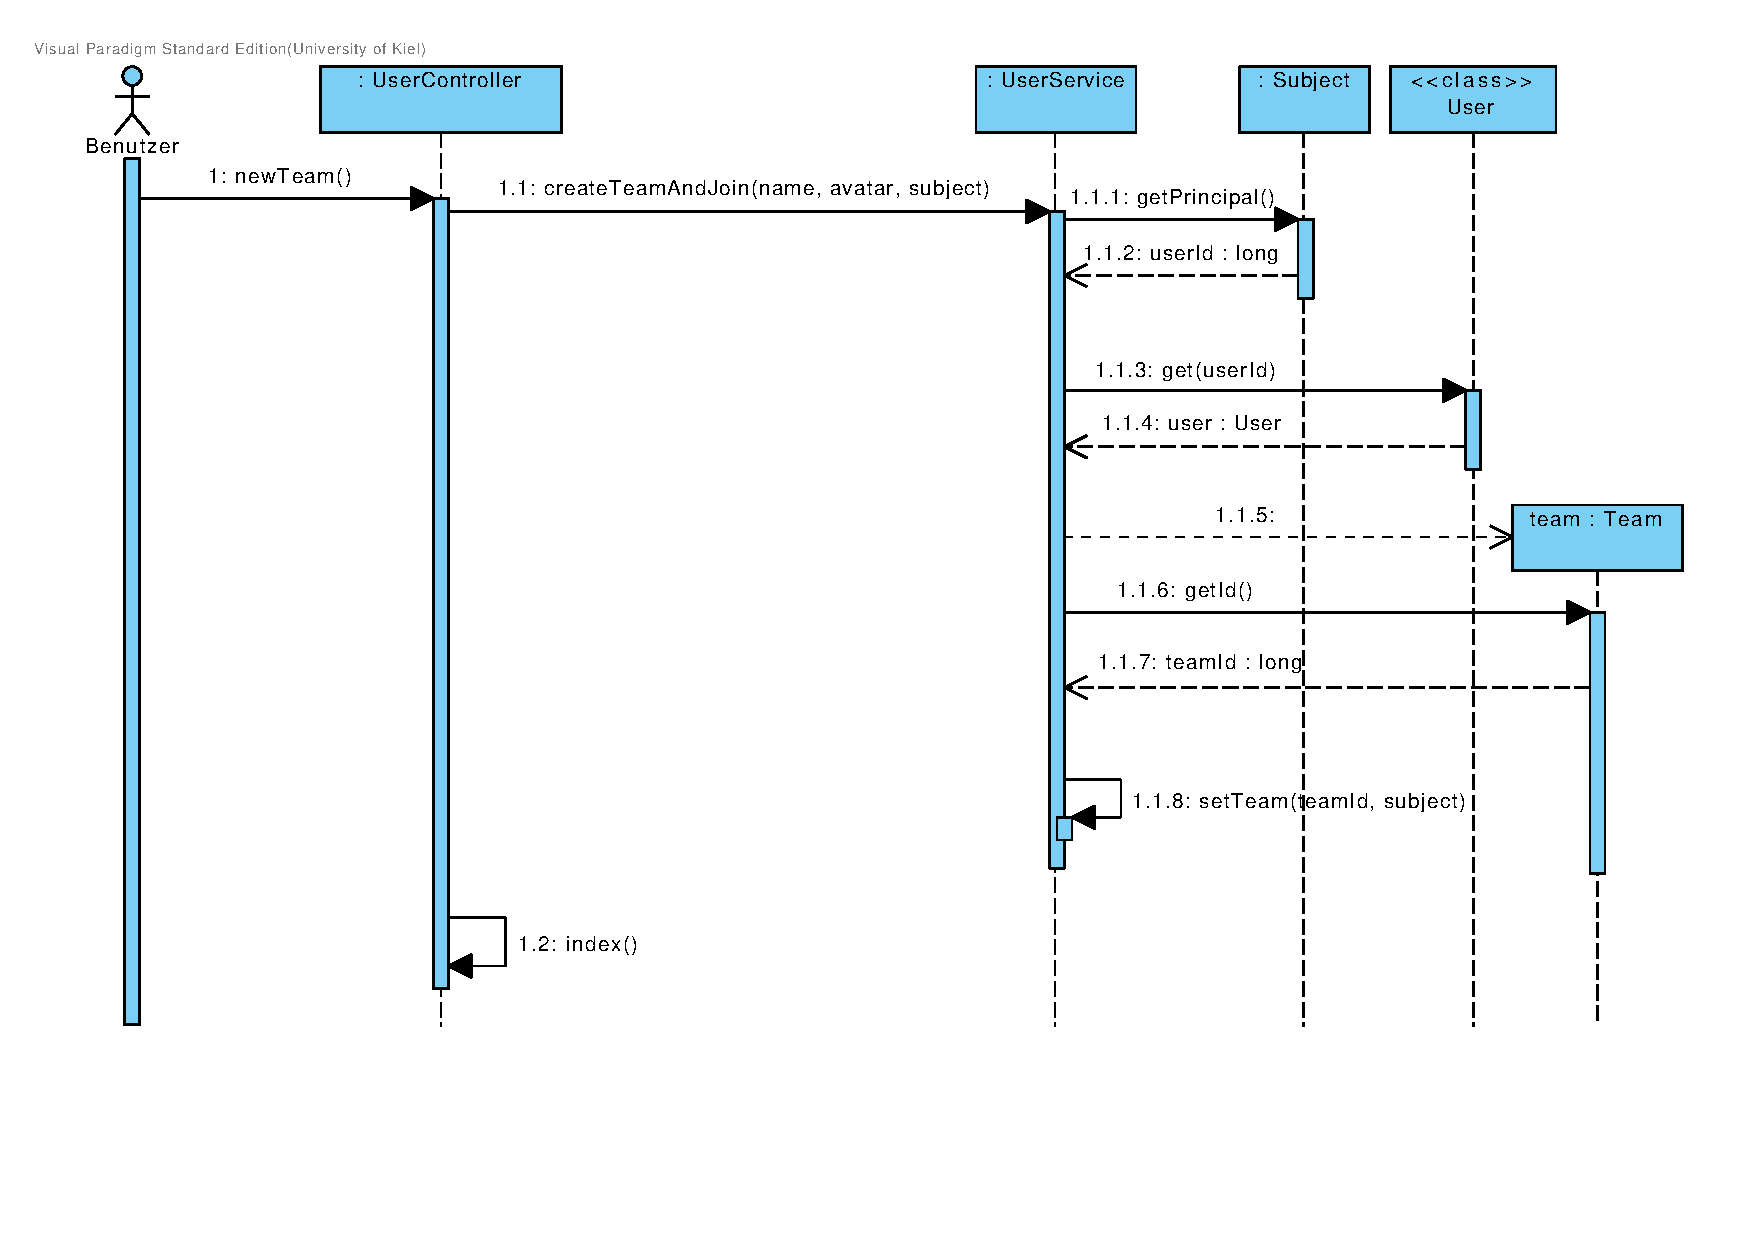
\includegraphics[width=\textwidth, clip]{gfx/team_erstellen}
  \caption{Ein Team erstellen}
\end{figure}

Der eingeloggte Benutzer, welcher noch kein Mitglied eines Teams ist,
kann auf seiner Landingpage über den Link „Team erstellen“ ein neues
Team generieren. Der Benutzer gelangt auf eine leere Teamprofilseite,
in der er den Teamnamen, ein Teamfoto und eine Beschreibung des Teams
eingeben kann. Anschließend bestätigt der Benutzer über einen Klick
auf „Team gründen“ sein Team. Mit der Bestätigung ist der Benutzer
automatisch dem Team beigetreten. Die Teamprofilseite aktualisiert
sich und der Benutzer sieht seine neue Teamprofilseite mit ihm als
Mitglied.\\

\subsection{Team blocken}
%TODO Image here
Der eingeloggte Admin kann ein Team über einen speziellen Button, welcher die Funktion blockTeam(teamId) aufruft, sperren. Dabei wird das Team und nacheinander jedes einzelne Teammitglied gesperrt. Nachdem dies geschehen ist, tauchen auch das Team und deren Mitglieder nicht mehr in der Teilnehmerliste auf.\\

\subsection{Vorschlag erstellen}
\begin{figure}[H]
  \centering
  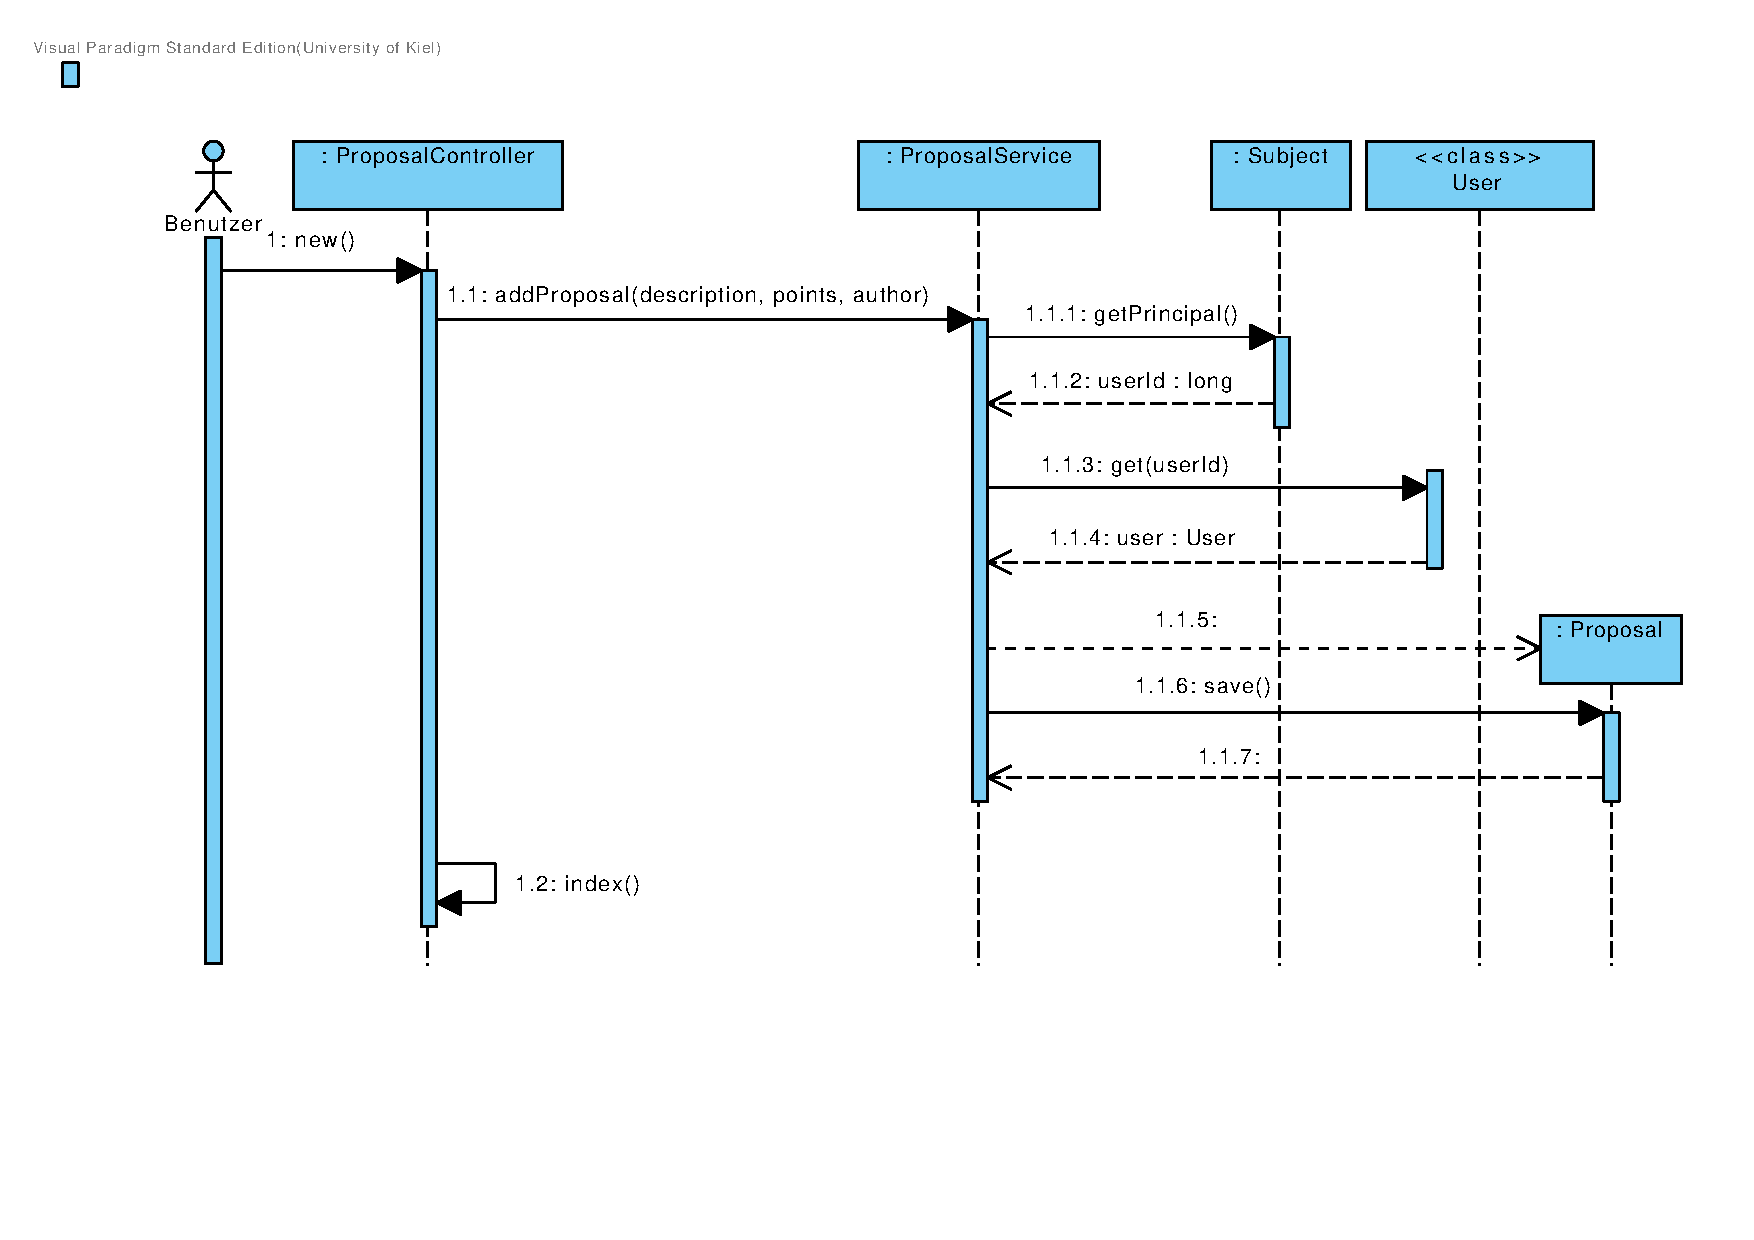
\includegraphics[width=\textwidth, clip]{gfx/vorschlag_erstellen}
  \caption{Einen Vorschlag erstellen}
\end{figure}

Der eingeloggte Benutzer, kann auf der Vorschlagsseite über den Link
``eine neue Aktivität vorschlagen'' einen neuen Vorschlag für eine
Aktivität einreichen. Der Benutzer gelangt über den Link auf eine
Seite, auf welcher er eine Beschreibung und eine Punktzahl für seinen Vorschlag
 eingeben kann. Auf dieser Seite kann der Benutzer durch Klick auf
 ``Vorschlag einreichen'' den Vorschlag einreichen. Anschließend sieht
 der Benutzer die Bestätigung ``Vorschlag erfolgreich eingereicht''
 und wird auf die Vorschlagsseite zurückgeleitet, wo er seinen
 Vorschlag einesehen kann.
 
\subsection{Vorschlag bewerten}
\begin{figure}[H]
  \centering
  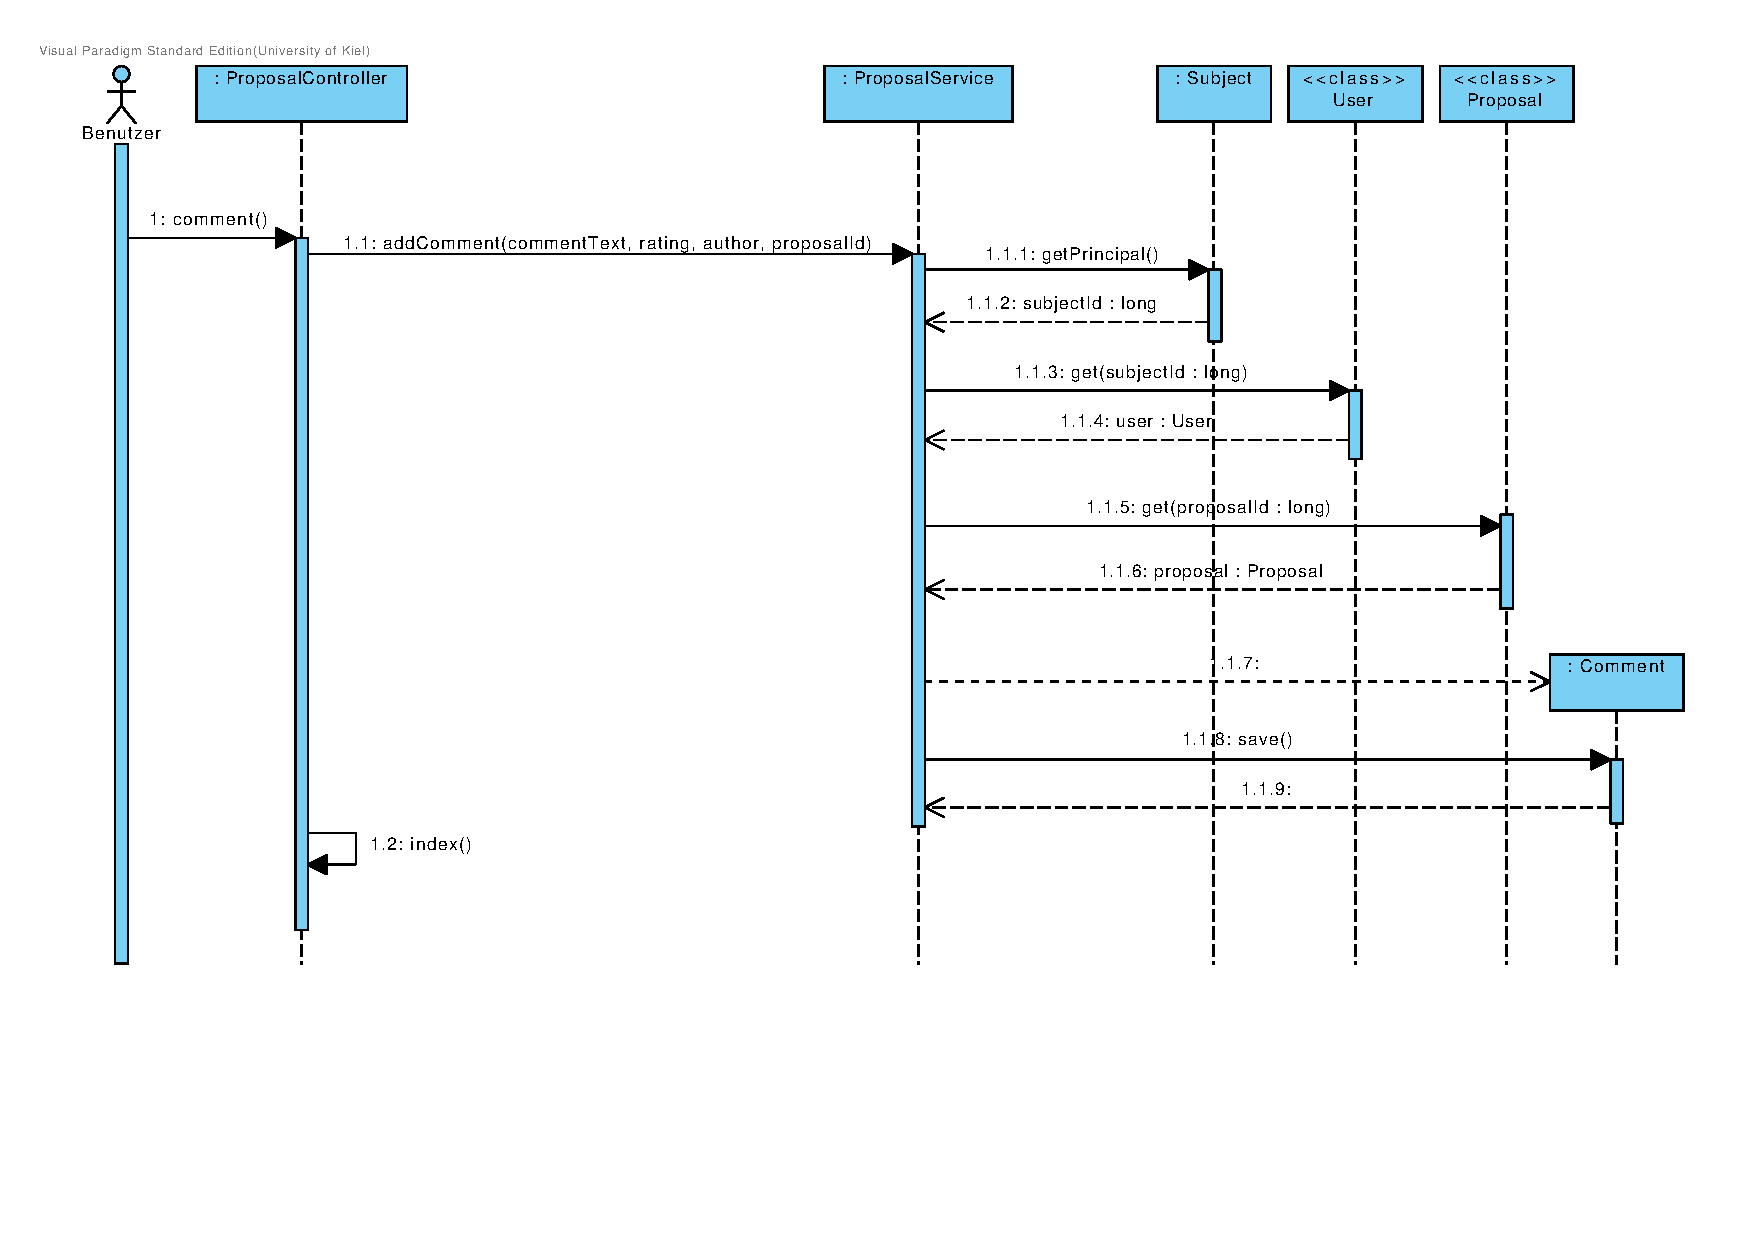
\includegraphics[width=\textwidth, clip]{gfx/vorschlag_bewerten}
  \caption{Einen Vorschlag bewerten}
\end{figure}

Der eingeloggte Benutzer, kann auf der Vorschlagsseite über den Link
``diesen Vorschlag bewerten'', welcher bei jedem Vorschlag angezeigt
wird, eine Bewertung zu jedem eingereichten Vorschlag abgeben. Durch
Klick auf diesen Link gelangt der Benutzer auf eine Seite, auf welcher
er ein Kommentar und/oder eine Bewertung in Form von 1 bis 5 Sternen
abgeben kann. Auf dieser Seite kann der Benutzer durch Klick auf
 ``Bewertung abgeben'' die Bewertung abgeben. Anschließend sieht
 der Benutzer die Bestätigung ``Bewertung abgegeben'' und wird auf die Vorschlagsseite zurückgeleitet.
 

\subsection{Statistiken exportieren}
%TODO Image here
Der eingeloggte Benutzer klickt auf Statistik und gelangt auf die Statistikseite, wo er auf den Button „Herunterladen“ klickt. Nun wird dem Benutzer ein Download zur Verfügung gestellt, welcher ihm ermöglicht, die Statistiken in einer „.csv“-Datei auf dem eigenen Computer zu speichern.\\
\subsection{Vorschlag in Aktivität umwandeln}
%TODO Image here
\subsection{App: Benutzerrangliste ansehen}
Die Serveranfragen in der App funktionieren alle nach dem selben Muster. Benutzerrangliste ansehen steht hier exemplarisch für weitere Anwendungsfälle dieser Art.
%TODO Image here
Wenn der Nutzer in der App zur Benutzerrangliste navigiert, wird diese automatisch bei der Erstellung des \emph{Fragments} geladen. Dabei wird auf ein \emph{GetUserRankingTask} die Methode \emph{execute()} aufgerufen. \emph{GetUserRankingTask} erbt von \emph{AccessServerTask}, die wiederum von der Androidklassse \emph{AsyncTask} erbt. In dem \emph{AccessServerTask} wird die Methode \emph{doInBackground()} aufgerufen, die wiederum die Methode \emph{createServerRequest} aufruft, die im \emph{GetUserRankingTask} definiert ist.\\
Sobald die \emph{doInBackground()}-Methode fertig ausgeführt wurde, wird (vom \emph{AsyncTask}) die Methode \emph{onPostExecute()} aufgerufen, die \emph{handleServerResponse()} des \emph{GetUserRankingTask} ausführt. Hier wird dann die Darstellung im \emph{Fragment} getätigt.\\
Der Vorteil dieser Art der Implementierung ist, dass nur einmal eine generelle Serverabfrage definiert werden muss, und sich keine weitere Gedanken um dessen Implementierung gemacht werden m\"ussen. Deswegen ist die Durchführung der HTTP-Abfrage hier auch nicht weiter aufgeführt.
\section{Anhang}
\subsection{Klassen Diagramme}

\begin{figure}[H]
  \centering
  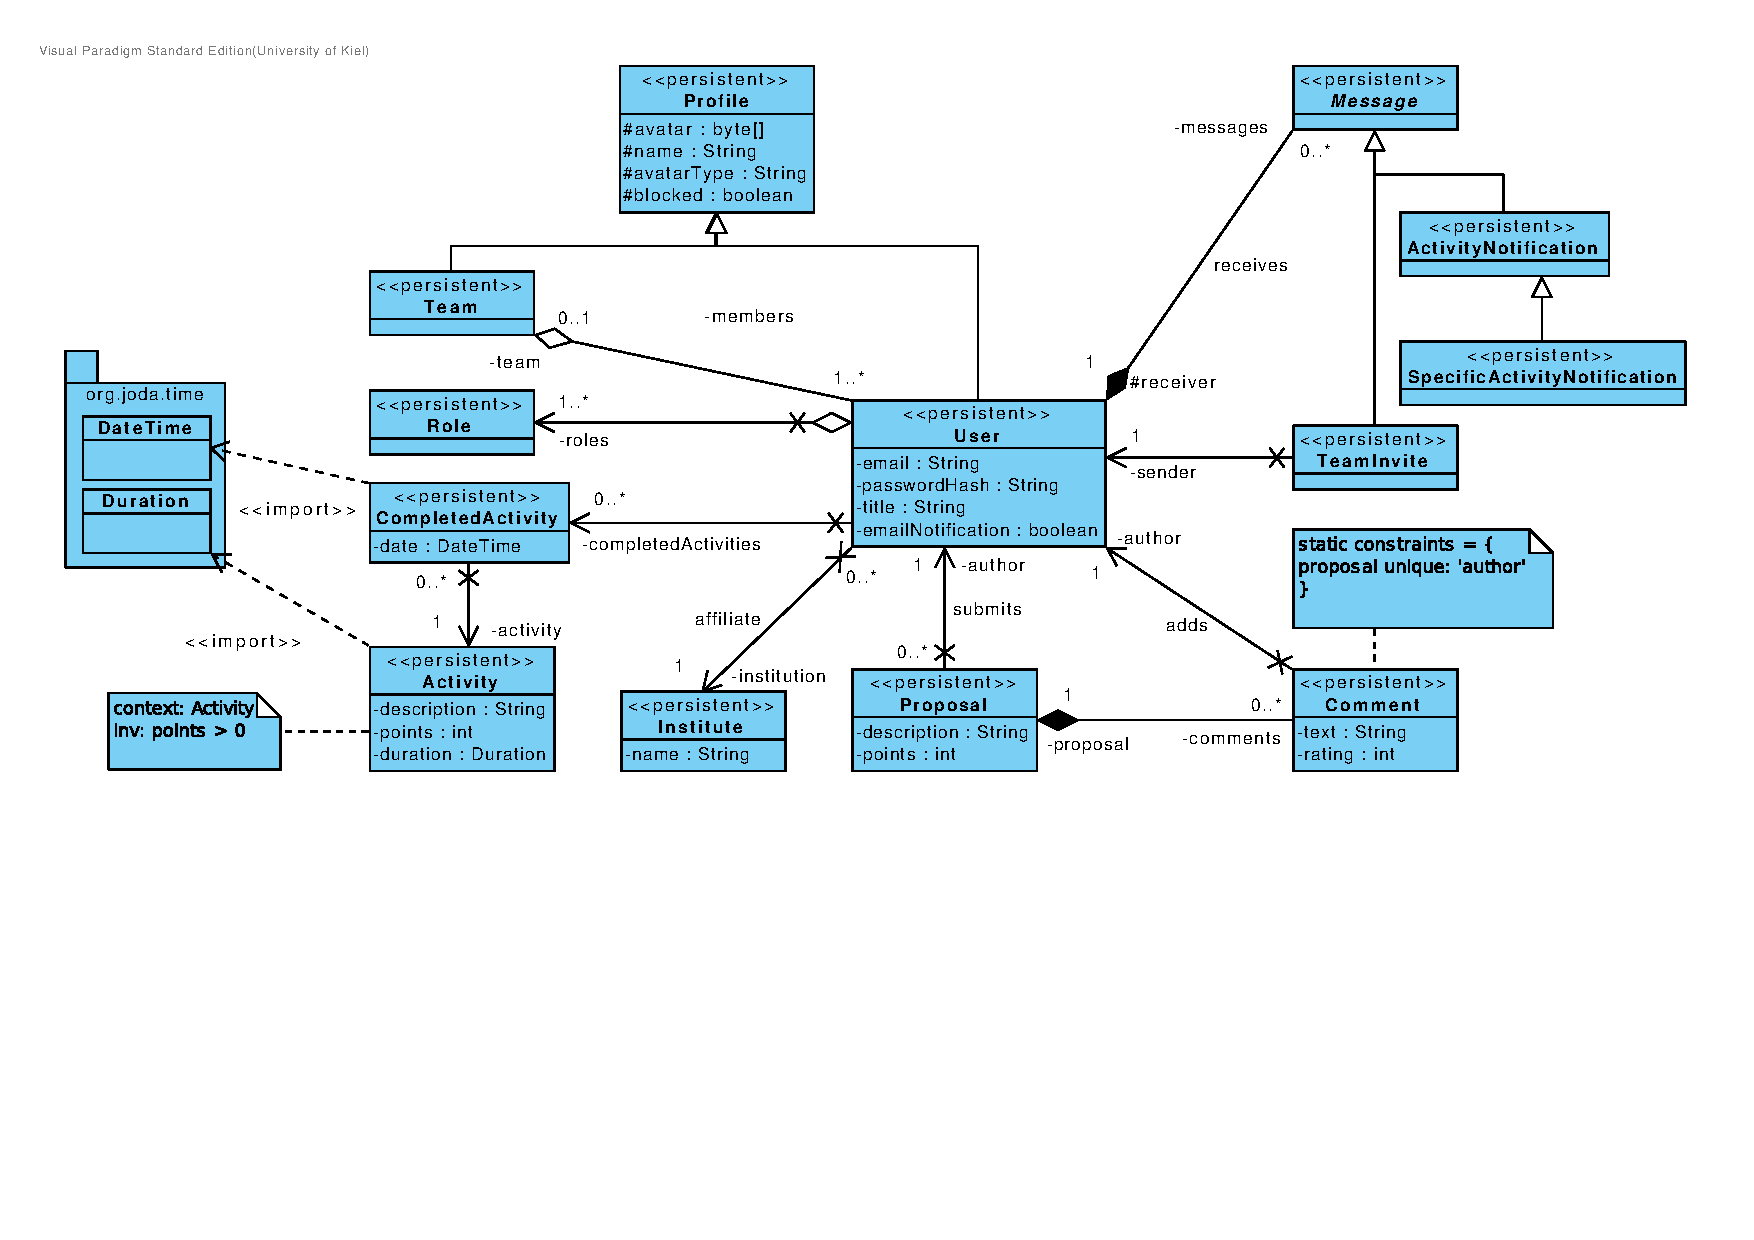
\includegraphics[width=\textwidth, trim=1cm 1cm 1cm 1cm, clip]{gfx/persistent_classes}
  \caption{Persistenzklassen}
\end{figure}

\begin{figure}[H]
  \centering
  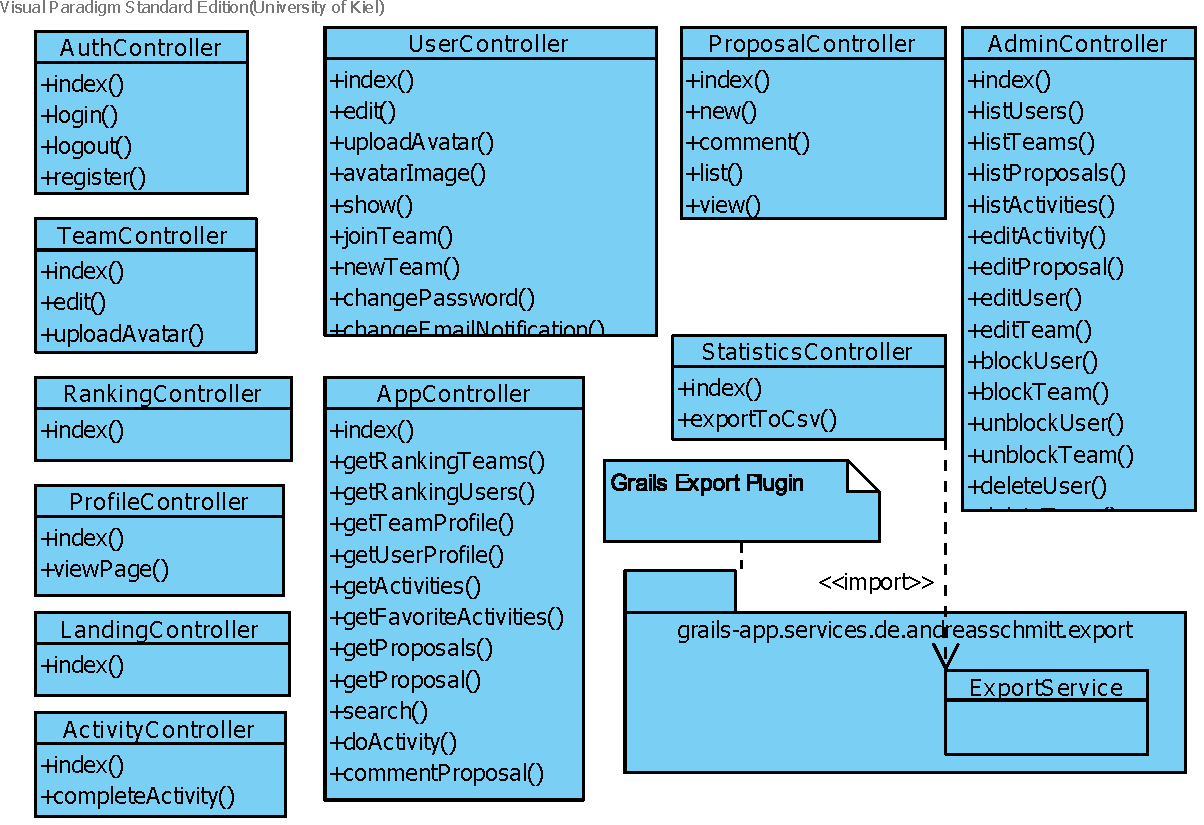
\includegraphics[width=\textwidth, trim=1cm 10cm 11cm 1cm, clip]{gfx/controller_classes}
  \caption{Contollerklassen}
\end{figure}

\begin{figure}[H]
  \centering
  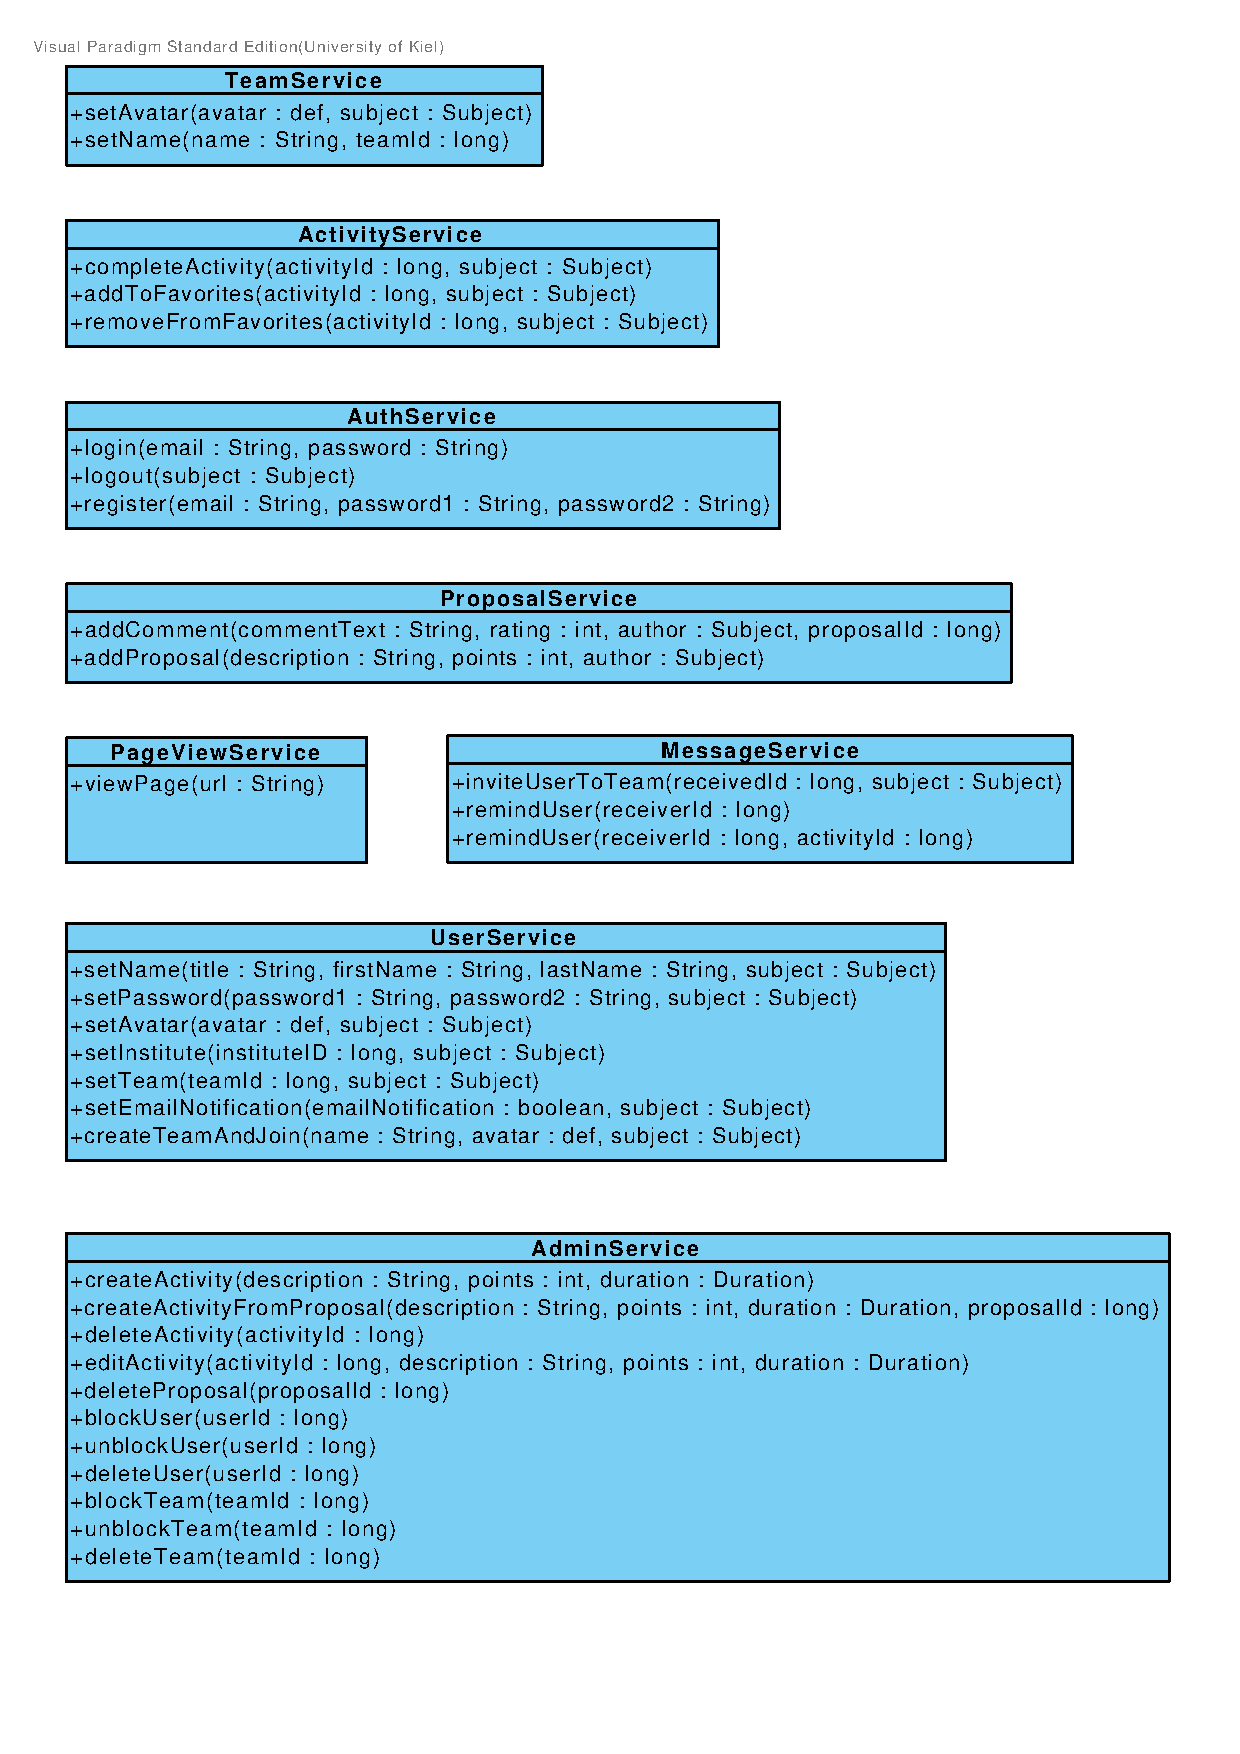
\includegraphics[width=\textwidth, trim=1cm 10cm 11cm 1cm, clip]{gfx/service_classes}
  \caption{Serviceklassen}
\end{figure}


\end{document}